\documentclass{article}

\title{\sc\LARGE CSCA67 Tutorial, Week 11\\
{\Large Nov. 23rd-Nov. 27th, 2015}}
\date{}
\author{\sc Compiled by {\em G. Singh Cadieux}\\[1ex]
\sc Adapted from\\
A. Bretscher, \href{http://www.utsc.utoronto.ca/~bretscher/a67/lectures/induction_ppt.pdf}{\em CSCA67 Week 10 Lecture Notes},\\
\href{http://youtu.be/NuGDkmwEObM?t=58m50s}{\em Lec 3 \textbar MIT 6.042J Mathematics for Computer Science, Fall 2010} \&\\
V. Hadzilacos, \textit{Course notes for {\em Introduction to the Theory of Computation}} (2007).}

\usepackage{fullpage}
\usepackage{amsmath,amssymb}
%\usepackage{color}
%\usepackage{multicol}
\usepackage{tikz}
\usepackage{hyperref}

\usetikzlibrary{patterns}
\usetikzlibrary{backgrounds}
\tikzstyle{background rectangle}=[draw=none]

\setlength{\parindent}{0pt}

\begin{document}
\maketitle

\section{\sc Review of last week's lecture}
\subsection*{\em Proof by induction}
Proof by induction is a proof technique that is used to prove that a predicate $P(n)$ is true for all natural numbers $n$ larger than $b$, where $b$ is a natural number.\\[1ex]
The natural numbers are the ``counting numbers": the nonnegative integers 0, 1, 2, \ldots (note that, depending upon the context, 0 may or may not be included in the natural numbers). The set of natural numbers is denoted $\mathbb{N}$.\\[1ex]
For example, suppose we have the predicate $P(n): n(n^2+5)$ is divisible by 6.\\
We can demonstrate that $P(n)$ is true or false for a specific value of $n$: for instance, if we choose $n=2$, $2(2^2+5)=18$ is divisible by 6, so $P(6)$ is true.\\
But we cannot demonstrate that $P(n)$ is true for all $n\in\mathbb{N}$ - that is, for all natural numbers $n$ - by successively choosing $n$ to be every natural number, since there are infinitely many natural numbers. We can instead use proof by induction to prove that $P(n)$ is true for all $n\in\mathbb{N}$.\\[1em]
\textsc{Proof Structure:}\\[1ex]
Establish a statement $S(n)$ to prove.\\
Generally, $S(n)$ will take the form ``$P(n)$ is true for all natural numbers $n\geq b$," where $P(n)$ is a predicate such as ``$n(n^2+5)$ is divisible by 6."
\begin{enumerate}
\item \textbf{Base case/basis:} Prove that $P(b)$ is true.
\item \textbf{Induction hypothesis:} Suppose that $P(k)$ is true for all natural numbers $k\geq b$.
\item \textbf{Induction step:} Prove that $P(k)$ implies $P(k+1)$ (i.e., prove that $P(k+1)$ is true if $P(k)$ is true).
\end{enumerate}
Conclude that $P(n)$ is true for all natural numbers $n\geq b$, which is to say that $S(n)$ is true.\\[1em]
\textsc{Intuitively}, this makes sense because, if $P(k)\to P(k+1)$, and $P(b)$ is true, then we reach each natural number with a series of implications starting from $b$:
\begin{equation*}
P(b)\to P(b+1)\to P((b+1)+1)\to P((b+2)+1)\to P((b+3)+1)\to\ldots
\end{equation*}

\textsc{Formally}, we can demonstrate that induction proofs are valid using the \textit{well-ordering principle}.\\[1ex]
\textbf{Well-Ordering Principle:} Any non-empty subset $C$ of $\mathbb{N}$ contains a smallest element.\\[1em]
Suppose that we have completed all 3 steps of a proof by induction in order to prove that $P(n)$ is true for all $n\in\mathbb{N}$ greater than $b$.\\[1ex]
Let $C=\{x\,|\,P(x)\text{ is false},\,x\geq b,\, x\in\mathbb{N}\}$ be the set of all values greater than $b$ for which $P(n)$ is false.\\[1ex]
Suppose that our proof is not valid. Then there must be at least one value for which $P(n)$ is false, so $C$ is non-empty. Then by the well-ordering principle, there exists a smallest element $a\in C$.\\[1ex]
Since our base case proves that $P(b)$ is true, $a\neq b$.\\[1ex]
Since $a>b$ and $b$ is a natural number, $a$ must be a natural number and $(a-1)$ must also be a natural number. But $(a-1)<a$ and $a$ is the smallest element in $C$, so $(a-1)$ must not be in $C$ - that is, $P(a-1)$ must be true.\\[1ex]
However, by the induction hypothesis, if $P(a-1)$ is true, then $P((a-1)+1)=P(a)$ must be true as well. Then $a$ is not in $C$.\\[1ex]
This is a contradiction, demonstrating that our assumption that $C$ is nonempty must be false. Since $C$ \textit{is} empty, there are no values for which $P(n)$ is false if the base case and induction hypothesis hold.\\[1em]
\textsc{Note} that a common misunderstanding of proof by induction is to think that, by using the induction hypothesis, our proof assumes that $P(n)$ is true for all natural numbers. This is \textit{not} the case.\\[1ex]
Rather, we use the induction hypothesis in the induction step to prove that, for any natural number $k$, \textit{if} $P(k)$ is true, then $P(k+1)$ is true as well. Recall that we can prove an implication $p\to q$ true if we prove that, when $p$ is true, $q$ is also true. We are not assuming that $P(n)$ is absolutely true; we are assuming that $P(n)$ is true only to prove that the implication $P(n)\to P(n+1)$ is true.\\[1em]
Q: \textsc{Prove that $P(n): 0+1+2+\ldots+(n-1)+n=\dfrac{n(n+1)}{2}$ is true for all $n\in\mathbb{N}$.}\\[1ex]
Let $S(n)$ be the statement that $P(n)$ holds for all $n\in\mathbb{N}$.\\[1ex]
\textbf{Basis:} $n=0$\\[1ex]
$\dfrac{(0)(0+1)}{2}=0$\\[1ex]
$\Rightarrow P(0)$ holds.\\[1ex]
\textbf{Induction hypothesis:} Suppose that $P(k)$ holds for $k\geq 0$.\\[1ex]
\textbf{Induction step:} $n=k+1$
\begin{align*}
0+1+2+\ldots+k+(k+1)& =(0+1+2+\ldots+k)+(k+1)\\
& =\dfrac{k(k+1)}{2}+(k+1)& \text{[by the induction hypothesis]}\\
& =\dfrac{k(k+1)}{2}+\dfrac{2(k+1)}{2}\\
& =\dfrac{(k+2)(k+1)}{2}\\
& =\dfrac{(k+1)((k+1)+1)}{2}
\end{align*}
$\Rightarrow P(k+1)$ holds if $P(k)$ holds, for $k\geq 0$.\\[1ex]
$\boxed{\Rightarrow S(n)\text{ is true.}}$

\section{\sc Proof by simple induction}

\subsection*{\href{http://www.youtube.com/watch?v=IFqna5F0kW8}{Q: {\em Prove that $4+9+14+19+\ldots+(5n-1)=\dfrac{n}{2}(3+5n)$ for all natural numbers $n$.}}}

Let $P(n)$ be the predicate ``$4+9+14+19+\ldots+(5n-1)=\tfrac{n}{2}(3+5n)$".\\
Let $S(n)$ be the statement that $P(n)$ holds for all $n\in\mathbb{N}$ (note that, here, $0\notin\mathbb{N}$).\\[1ex]
\textbf{Basis:} $n=1$\\[1ex]
$5(1)-1=4$\\[1ex]
$\dfrac{1}{2}(3+5(1))=\dfrac{1}{2}(8)=4$\\[1ex]
$5(1)-1=\dfrac{1}{2}(3+5(1))\Rightarrow P(1)$ holds.\\[1ex]
\textbf{Induction hypothesis:} Suppose that $P(k)$ holds for $k\geq 1$.\\[1ex]
\textbf{Induction step:} $n=k+1$
\begin{align*}
4+9+14+19+\ldots+(5(k)-1)+(5(k+1)-1)& =\dfrac{k}{2}(3+5(k))+(5(k+1)-1)& \text{[by I.H.]}\\
& =\dfrac{5}{2}k^2+\dfrac{13}{2}k+4& \text{[expanded and simplified]}\\
\dfrac{(k+1)}{2}(3+5(k+1))& =\left(\dfrac{k}{2}+\dfrac{1}{2}\right)(3+5k+5)\\
& =(\dfrac{5}{2}k^2+4k)+(\dfrac{5}{2}+4)& \text{[expanded and simplified]}\\
4+9+14+19+\ldots+(5(k)-1)+(5(k+1)-1)& =\dfrac{(k+1)}{2}(3+5(k+1))
\end{align*}
$\Rightarrow P(k+1)$ holds if $P(k)$ holds, for $k\geq 1$.\\[1ex]
$\boxed{\Rightarrow S(n)\text{ is true.}}$

\subsection*{\href{http://www.youtube.com/watch?v=wBvsIyQN4o8}{Q: {\em Prove that $-1+2+5+8+\ldots+(3n-4)=\dfrac{n}{2}(3-5n)$ for all natural numbers $n$.}}}

Let $P(n)$ be the predicate ``$-1+2+5+8+\ldots+(3n-4)=\tfrac{n}{2}(3-5n)$".\\
Let $S(n)$ be the statement that $P(n)$ holds for all $n\in\mathbb{N}$ (note that, here, $0\notin\mathbb{N}$).\\[1ex]
\textbf{Basis:} $n=1$\\[1ex]
$3(1)-4=-1$\\[1ex]
$\dfrac{1}{2}(3-5(1))=\dfrac{1}{2}(-2)=-1$\\[1ex]
$3(1)-4=\dfrac{1}{2}(3-5(1))\Rightarrow P(1)$ holds.\\[1ex]
\textbf{Induction hypothesis:} Suppose that $P(k)$ holds for $k\geq 1$.\\[1ex]
\textbf{Induction step:} $n=k+1$
\begin{align*}
-1+2+5+8+\ldots+(3(k)+4)+(3(k+1)-4)& =\dfrac{k}{2}(3-5(k))+(3(k+1)-4)& \text{[by I.H.]}\\
& =\dfrac{3}{2}k^2+\dfrac{1}{2}k-1& \text{[expanded and simplified]}\\
\dfrac{(k+1)}{2}(3+5(k+1))& =\left(\dfrac{k}{2}+\dfrac{1}{2}\right)(3+5k+5)\\
& =\dfrac{3}{2}k^2+\dfrac{1}{2}k-1& \text{[expanded and simplified]}\\
-1+2+5+8+\ldots+(3(k)+4)+(3(k+1)-4)& =\dfrac{(k+1)}{2}(3+5(k+1))
\end{align*}
$\Rightarrow P(k+1)$ holds if $P(k)$ holds, for $k\geq 1$.\\[1ex]
$\boxed{\Rightarrow S(n)\text{ is true.}}$

\subsection*{\href{http://www.youtube.com/watch?v=uHfwNKWyD20}{Q: {\em Prove that $\dfrac{1}{2}+\dfrac{1}{4}+\dfrac{1}{8}+\ldots+\dfrac{1}{2^n}=\dfrac{2^n-1}{2^n}$ for all natural numbers $n$.}}}

Let $P(n)$ be the predicate ``$\tfrac{1}{2}+\tfrac{1}{4}+\tfrac{1}{8}+\ldots+\tfrac{1}{2^n}=\tfrac{2^n-1}{2^n}$".\\
Let $S(n)$ be the statement that $P(n)$ holds for all $n\in\mathbb{N}$ (note that, here, $0\notin\mathbb{N}$).\\[1ex]
\textbf{Basis:} $n=1$\\[1ex]
$\dfrac{1}{2^{(1)}}=\dfrac{1}{2}$\\[1ex]
$\dfrac{2^{(1)}-1}{2^{(1)}}=\dfrac{1}{2}$\\[1ex]
$\dfrac{1}{2^{(1)}}=\dfrac{2^{(1)}-1}{2^{(1)}}\Rightarrow P(1)$ holds.\\[1ex]
\textbf{Induction hypothesis:} Suppose that $P(k)$ holds for $k\geq 1$.\\[1ex]
\textbf{Induction step:} $n=k+1$
\begin{align*}
\dfrac{1}{2}+\dfrac{1}{4}+\dfrac{1}{8}+\ldots+\dfrac{1}{2^{(k)}}+\dfrac{1}{2^{(k+1)}}& =\dfrac{2^k-1}{2^k}+\dfrac{1}{2^{(k+1)}}& \text{[by I.H.]}\\
& =\dfrac{2(2^k-1)}{2^{(k+1)}}+\dfrac{1}{2^{(k+1)}}\\
& =\dfrac{2^{(k+1)}-2}{2^{(k+1)}}+\dfrac{1}{2^{(k+1)}}\\
& =\dfrac{2^{(k+1)}-1}{2^{(k+1)}}
\end{align*}
$\Rightarrow P(k+1)$ holds if $P(k)$ holds, for $k\geq 1$.\\[1ex]
$\boxed{\Rightarrow S(n)\text{ is true.}}$

\section{\sc Proof by complete induction}
So far, we have been using a type of proof by induction known as ``simple" induction. Another type of proof by induction is \textit{complete} (or \textit{strong}) induction.\\[1ex]
Like simple induction, complete induction is used to prove that a predicate $P(n)$ is true for all natural numbers $n$ larger than $b$, where $b$ is a natural number.\\[1ex]
The difference betwen the two techniques is in the induction hypothesis: rather than assuming only that $P(k)$ is true, we assume that $P(b),\,P(b+1),\,P(b+2),\,\ldots,\,P(k)$ are all true (a ``stronger" induction hypothesis, hence the name of the technique).\\[1ex]
It is easier to use complete induction than simple induction for certain problems, since there are more assumptions that we can use.\\[1em]
\textsc{Proof Structure:}\\[1ex]
Establish a statement $S(n)$ to prove.\\
Generally, $S(n)$ will take the form ``$P(n)$ is true for all natural numbers $n\geq b$," where $P(n)$ is a predicate such as ``$n(n^2+5)$ is divisible by 6."
\begin{enumerate}
\item \textbf{Base case/basis:} Prove that $P(b)$ is true.
\item \textbf{Induction hypothesis:} Suppose that $P(b+1),\,P(b+2),\,\ldots,\,P(k)$ are true for all natural numbers $k\geq b$.
\item \textbf{Induction step:} Prove that $P(b)\wedge P(b+1)\wedge P(b+2)\wedge\ldots\wedge P(k)$ implies $P(k+1)$ (i.e., prove that $P(k+1)$ is true if $P(b),\,P(b+1),\,P(b+2),\,\ldots,\,P(k)$ are true).
\end{enumerate}
Conclude that $P(n)$ is true for all natural numbers $n\geq b$, which is to say that $S(n)$ is true.

\subsection*{\em The Unstacking Game}
Consider a game in which each player starts off with a stack of objects.

\begin{itemize}
\item At his/her turn, each player splits (one of) his/her stack(s) into 2 smaller stacks.
\item The number of points for each turn is the product of the sizes of the 2 stacks.
\item The players continue taking turns and splitting their stacks until all the stacks contain only 1 object each.
\item Each player's total score is the sum of his/her scores for all the turns. The player with the largest total score is the winner.
\end{itemize}
For example, starting with 5 objects, one possible strategy is:\\
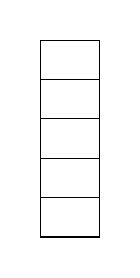
\begin{tikzpicture}[framed, inner frame sep=1ex]
\draw (0,0) rectangle (0.75,0.5);
\draw (0,0.5) rectangle (0.75,1);
\draw (0,1) rectangle (0.75,1.5);
\draw (0,1.5) rectangle (0.75,2);
\draw (0,2) rectangle (0.75,2.5);
\end{tikzpicture}
\begin{tikzpicture}[framed, inner frame sep=1ex]
\draw (0,0) rectangle (0.75,0.5);
\draw (0,0.5) rectangle (0.75,1);
\draw (0.85,0) rectangle (1.6,0.5);
\draw (0.85,0.5) rectangle (1.6,1);
\draw (0.85,1) rectangle (1.6,1.5);
\end{tikzpicture}
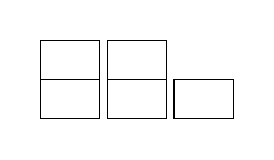
\begin{tikzpicture}[framed, inner frame sep=1ex]
\draw (0,0) rectangle (0.75,0.5);
\draw (0,0.5) rectangle (0.75,1);
\draw (0.85,0) rectangle (1.6,0.5);
\draw (0.85,0.5) rectangle (1.6,1);
\draw (1.7,0) rectangle (2.45,0.5);
\end{tikzpicture}
\begin{tikzpicture}[framed, inner frame sep=1ex]
\draw (-0.85,0) rectangle (-0.1,0.5);
\draw (0,0) rectangle (0.75,0.5);
\draw (0.85,0) rectangle (1.6,0.5);
\draw (0.85,0.5) rectangle (1.6,1);
\draw (1.7,0) rectangle (2.45,0.5);
\end{tikzpicture}
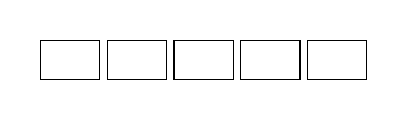
\begin{tikzpicture}[framed, inner frame sep=1ex]
\draw (0,0) rectangle (0.75,0.5);
\draw (0.85,0) rectangle (1.6,0.5);
\draw (1.7,0) rectangle (2.45,0.5);
\draw (2.55,0) rectangle (3.3,0.5);
\draw (3.4,0) rectangle (4.15,0.5);
\end{tikzpicture}\\
This player will have $(2\times 3)+(2\times 1)+(1\times 1)+(1\times 1)=10$ points in total.\\[1em]
When we play the unstacking game, however, we notice that all strategies appear to result in the same score. For example, here is another strategy when starting with a stack of 5 objects:\\
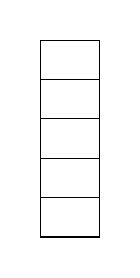
\begin{tikzpicture}[framed, inner frame sep=1ex]
\draw (0,0) rectangle (0.75,0.5);
\draw (0,0.5) rectangle (0.75,1);
\draw (0,1) rectangle (0.75,1.5);
\draw (0,1.5) rectangle (0.75,2);
\draw (0,2) rectangle (0.75,2.5);
\end{tikzpicture}
\begin{tikzpicture}[framed, inner frame sep=1ex]
\draw (0,0) rectangle (0.75,0.5);
\draw (0.85,0) rectangle (1.6,0.5);
\draw (0.85,0.5) rectangle (1.6,1);
\draw (0.85,1) rectangle (1.6,1.5);
\draw (0.85,1.5) rectangle (1.6,2);
\end{tikzpicture}
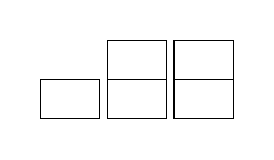
\begin{tikzpicture}[framed, inner frame sep=1ex]
\draw (0,0) rectangle (0.75,0.5);
\draw (0.85,0) rectangle (1.6,0.5);
\draw (0.85,0.5) rectangle (1.6,1);
\draw (1.7,0) rectangle (2.45,0.5);
\draw (1.7,0.5) rectangle (2.45,1);
\end{tikzpicture}
\begin{tikzpicture}[framed, inner frame sep=1ex]
\draw (-0.85,0) rectangle (-0.1,0.5);
\draw (0,0) rectangle (0.75,0.5);
\draw (0.85,0) rectangle (1.6,0.5);
\draw (0.85,0.5) rectangle (1.6,1);
\draw (1.7,0) rectangle (2.45,0.5);
\end{tikzpicture}
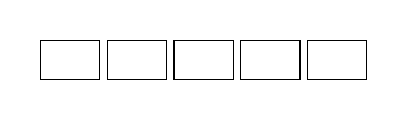
\begin{tikzpicture}[framed, inner frame sep=1ex]
\draw (0,0) rectangle (0.75,0.5);
\draw (0.85,0) rectangle (1.6,0.5);
\draw (1.7,0) rectangle (2.45,0.5);
\draw (2.55,0) rectangle (3.3,0.5);
\draw (3.4,0) rectangle (4.15,0.5);
\end{tikzpicture}\\
This again produces a total score of $(1\times 4)+(1\times 3)+(2\times 1)+(1\times 1)=10$ points.\\[1em]
\textsc{We can theorize} that, for an inital stack of $n$ objects, any strategy will produce the same score $S(n)$. And since we believe that all strategies produce the same score, let us choose a strategy and calculate the resulting score $S(n)$, which should result from any other strategy as well.\\[1ex]
We know (and have demonstrated above) that the sum of all natural numbers up to $n$ is $\tfrac{n(n+1)}{2}$. If we choose the strategy of splitting each stack of blocks into a stack of 1 block and a stack of all the remaining blocks, then our total score will be $((n-1)\times 1)+(((n-1)-1)\times 1)+\ldots+(1\times 1)=(n-1)+(n-2)+\ldots+1$.\\
For example, when starting with 5 objects, our strategy proceeds as follows:\\
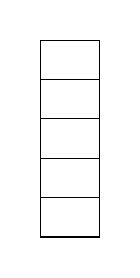
\begin{tikzpicture}[framed, inner frame sep=1ex]
\draw (0,0) rectangle (0.75,0.5);
\draw (0,0.5) rectangle (0.75,1);
\draw (0,1) rectangle (0.75,1.5);
\draw (0,1.5) rectangle (0.75,2);
\draw (0,2) rectangle (0.75,2.5);
\end{tikzpicture}
\begin{tikzpicture}[framed, inner frame sep=1ex]
\draw (0,0) rectangle (0.75,0.5);
\draw (0,0.5) rectangle (0.75,1);
\draw (0,1) rectangle (0.75,1.5);
\draw (0,1.5) rectangle (0.75,2);
\draw (0.85,0) rectangle (1.6,0.5);
\end{tikzpicture}
\begin{tikzpicture}[framed, inner frame sep=1ex]
\draw (0,0) rectangle (0.75,0.5);
\draw (0,0.5) rectangle (0.75,1);
\draw (0,1) rectangle (0.75,1.5);
\draw (0.85,0) rectangle (1.6,0.5);
\draw (1.7,0) rectangle (2.45,0.5);
\end{tikzpicture}
\begin{tikzpicture}[framed, inner frame sep=1ex]
\draw (0,0) rectangle (0.75,0.5);
\draw (0,0.5) rectangle (0.75,1);
\draw (0.85,0) rectangle (1.6,0.5);
\draw (1.7,0) rectangle (2.45,0.5);
\draw (2.55,0) rectangle (3.3,0.5);
\end{tikzpicture}
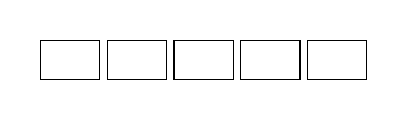
\begin{tikzpicture}[framed, inner frame sep=1ex]
\draw (0,0) rectangle (0.75,0.5);
\draw (0.85,0) rectangle (1.6,0.5);
\draw (1.7,0) rectangle (2.45,0.5);
\draw (2.55,0) rectangle (3.3,0.5);
\draw (3.4,0) rectangle (4.15,0.5);
\end{tikzpicture}\\
This gives us a score of $(4\times 1)+(3\times 1)+(2\times 1)+(1\times 1)=4+3+2+1$.\\[1ex]
In general, our total score from this strategy will be the sum of all natural numbers up to $(n-1)$, which we know to be $\tfrac{(n-1)((n-1)+1)}{2}=\tfrac{n(n-1)}{2}$.\\[1em]
\textsc{So now} let us use complete induction to prove\\
$Q(n):$ all strategies for the unstacking game produce the same score $S(n)=\dfrac{n(n-1)}{2}$ for all $n\in\mathbb{N}$, where $n$ is the number of objects in the initial stack.\\[1em]
\textbf{Basis:} $n=1$\\[1ex]
$S(1)=\dfrac{(1)((1)-1)}{2}=0$\\[1ex]
Since there are no moves that can be made with a stack of 1 object, all strategies will produce a score of 0. $\Rightarrow$ With $n=1$, all strategies produce the same score $S(1)$.\\[1ex]
\textbf{Induction hypothesis:} Suppose that, with $n=2$, all strategies produce the same score $S(2)$; with $n=3$, all strategies produce the same score $S(3)$; etc. Finally, suppose that, with $n=k\geq 1$, all strategies produce the same score $S(k)$.\\[1ex]
\textbf{Induction step:} $n=k+1$\\[1ex]
For our first turn, we divide the stack of $(k+1)$ objects into a stack of $m$ objects and a stack of $(k+1-m)$ objects (the value of $m$ depends upon our strategy).\\[1ex]
Based on our induction hypothesis, with an initial stack of $m\leq k$ objects, all strategies will produce a score of $S(m)=\tfrac{m(m-1)}{2}$; and with an initial stack of $(k+1-m)$ objects, all strategies will produce a score of $S(k+1-m)=\tfrac{(k+1-m)((k+1-m)-1)}{2}$.\\[1ex]
\textsc{Notice} that these assumptions cannot be used in simple induction.\\[1ex]
Then the total score for the game is the sum of the score for our first turn, and the total score for unstacking $m$ objects, and the total score for unstacking $(k+1-m)$ objects:
\begin{align*}
m(k+1-m)+S(m)+S(k+1-m)& =m(k+1-m)+\dfrac{m(m-1)}{2}+\dfrac{(k+1-m)((k+1-m)-1)}{2}\\
& =(km+m-m^2)+\dfrac{m^2-m}{2}+\dfrac{(k+1-m)(k+m)}{2}\\
& =\dfrac{1}{2}k^2+\dfrac{1}{2}k\qquad\text{[expanded and simplified]}
\end{align*}
Notice that this total score depends only on $k$ and not $m$ - that is, the total score depends only on the inital number of objects and not on our strategy, as we expected.
\begin{align*}
\dfrac{(k+1)((k+1)-1)}{2}& =\dfrac{k(k+1)}{2}\\
& =\dfrac{1}{2}k^2+\dfrac{1}{2}k\qquad\text{[expanded]}\\
m(k+1-m)+S(m)+S(k+1-m)& =\dfrac{(k+1)((k+1)-1)}{2}
\end{align*}
$\Rightarrow$ If all strategies produce the same score $S(2)$ with $n=2$, all strategies produce the same score $S(3)$ with $n=3$, etc., and all strategies produce the same score $S(k)$ with $n=k\geq 1$, then all strategies produce the same score $S(k+1)=\tfrac{(k+1)((k+1)-1)}{2}$ with $n=k+1$.\\[1ex]
$\boxed{\Rightarrow Q(n)\text{ is true.}}$

\section{\sc Additional practice problems}

{\bf Q: Using simple induction, prove that $1+2+4+\ldots+2^n=2^{n+1}-1$ for all natural numbers $n$.}\\[1em]
{\bf Q: Using simple induction, prove that $2^n\geq n^2$ for all natural numbers $n$.}\\[1em]
{\bf Q: Using simple induction, prove that $\sum\limits_{i=0}^n m^i=\dfrac{m^{n+1}-1}{m-1}$ for all integers $m\geq 2,\,n\geq 1$.}\\[1em]
Define the sequence $a_0,\,a_1,\,\ldots$ as\\
$a_i=\begin{cases}
2&\text{if }0\leq i\leq 2\\
a_{i-1}+a_{i-2}+a_{i-3}&\text{if }i>2
\end{cases}$\\[1ex]
{\bf Q: Using complete induction, prove that $a_n<2^n$ for every integer $n\geq 2$.}\\[1em]
{\bf Q: Find the flaw in the following proof by induction (a well-known proof by George P\'{o}lya).}\\[1ex]
$P(n)$: $n$ horses are of the same colour\\[1ex]
$S(n)$: $\forall n \in N$, $P(n)$ holds.\\[1ex]
\underline{Basis:} $n=1$\\[1ex]
$P(1)$ clearly holds as a single horse is the same colour as itself.\\[1ex]
\underline{Induction hypothesis:} Suppose that, within any set of $k$ horses, $k\geq 1$, all horses are of the same colour.\\[1ex]
\underline{Induction step:} $n=k+1$\\[1ex]
Consider a set of $k+1$ horses and number them $\{1,\,2,\,\ldots,\,k+1\}$ so that each horse is distinct. This set contains (among others) the overlapping subsets $\{1,\,2,\,\ldots,\,k\}$ and $\{2,\,3,\,\ldots,\,k+1\}$, each of which has $k$ horses.\\[1ex]
By the inductive hypothesis, the horses in the first subset are all of the same colour, and the horses in the second subset are all of the same colour. Both subsets contain the horses $\{2,\,3,\,\ldots,\,k\}$, meaning that these horses must all be of the same colour, and the horses not contained in both subsets (horse 1 in the first and horse $k+1$ in the second) must also be of the same colour as the rest. Thus, all $k+1$ horses are of the same colour.\\[1ex]
$\Rightarrow P(k+1)$ holds if $P(k)$ holds, for $k\geq 1$.\\[1ex]
$\boxed{\Rightarrow S(n)\text{ is true: all horses are of the same colour!}}$\\[1em]

{\bf Q: Find the flaw in the following proof by induction.}\\[1ex]
$P(n)$: $n=1$.\\[1ex]
$S(n)$: For all natural numbers $n\geq 1$, $P(n)$ holds.\\[1ex]
\underline{Basis:} $n=1$\\[1ex]
Trivial. $\Rightarrow P(1)$ holds.\\[1ex]
\underline{Induction hypothesis:} Suppose that $P(k)$ holds for $k\geq 1$ - that is, suppose that, for any $k\geq 1$, $k=1$.\\[1ex]
\underline{Induction step:} $n=k+1$\\[1ex]
Consider the (as yet unproven) statement $k+1=1$.
\begin{align*}
k+1& =1\\
(k+1)(k-1)& =1(k-1)\\
k^2-1& =k-1\\
k^2& =k\\
1^2& =1\qquad\text{[by I.H.]}
\end{align*}
Since this final statement is true, and is equivalent to the initial statement $k+1=1$, $k+1=1$ must be true as well.\\[1ex]
$\Rightarrow P(k+1)$ holds if $P(k)$ holds, for $k\geq 1$.\\[1ex]
$\boxed{\Rightarrow S(n)\text{ is true.}}$

\end{document}